% Define block styles
\tikzstyle{process} = [rectangle, draw, fill=blue!15, 
text width=9em, text centered, rounded corners, minimum height=6em, text width=4.6em]
\tikzstyle{line} = [draw, -latex', ultra thick]


\begin{tikzpicture}
% Place nodes

%-----------------------------------------------------------------------
\node [process, fill=red!10] (HM) {Heart Model};
\node [process, right of = HM, fill=red!20,  node distance = 4.3cm] (Int) {Interface};
\node [process, right of = Int, fill=red!30, node distance = 4.3cm] (PM) {Pacemaker};

%-----------------------------------------------------------------------




%\node[draw, dashed, inner sep=0.2cm,
%	label={[label distance=0cm]60:Section~\ref{sec:SHA}}, 
%	fit= (GFSM)(CC)] (S3) {};

%--------------------------------------------------------------------------------
%edges
\draw [line] (HM.40) -- (Int.140) node[midway, above,text width=2cm]
{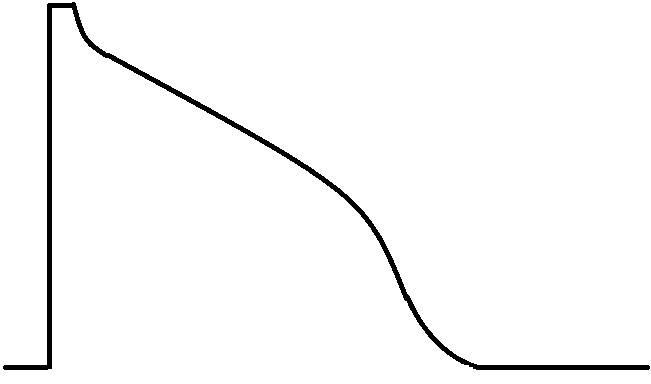
\includegraphics[scale=0.1]{figures/APicon}  Action Potentials };
\draw [line] (Int.40) -- (PM.140) node[midway, above,text width=2cm]
{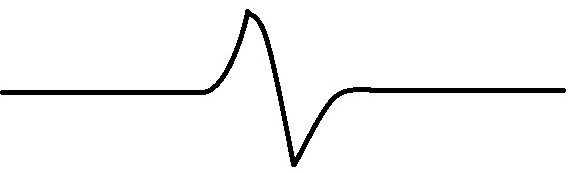
\includegraphics[scale=0.1]{figures/EGMicon} \acf{EGM}};
\draw [line] (PM.220) -- (Int.-40) node[midway, below,text width=2cm]
{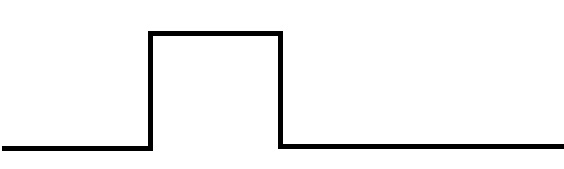
\includegraphics[scale=0.1]{figures/SQRicon} {Pacing}};
\draw [line] (Int.220) -- (HM.-40) node[midway, below,text width=2cm]
{Pacing};



\end{tikzpicture}    